
\documentclass[miz,woman]{mgrwms}
\usepackage[utf8x]{inputenc}
\usepackage{amsfonts}
\usepackage{amsmath}
\usepackage[polish]{babel}
\usepackage[T1]{fontenc}
\usepackage{mathptmx}
\usepackage{array}
\usepackage{amsthm}
\usepackage{graphicx}
\usepackage{eucal}



\title{ Twierdzenie Tur\`{a}na dla hipergrafów}
\author{ Agnieszka Walus}
\promotor{ prof zw. dr hab. Adam Paweł Wojda }
\nralbumu{ 124784 }
\slowakluczowe{ lista słów kluczowych w języku polskim }
\keywords{ lista słów kluczowych w języku angielskim }


\begin{document}
\newtheorem{defi}{Definicja}[chapter]
\newtheorem{hip}{Hipoteza}[chapter]
\newtheorem{tw}{Twierdzenie}[chapter]
\newtheorem{lem}[tw]{Lemat}
\theoremstyle{definition}
\newtheorem{przy}{Przykład}[chapter]
%\linespread{1.3}
%\maketitle
%\tableofcontents
%\begin{wstep}
 %Twierdzenie Mantela, a następnie twierdzenie Tur\'ana dla grafów spowodowało, że wielu matematyków zaczęło interesować się
%ekstremalną teorią grafów. W wyniku tego w drugiej połowie ubiegłego stulecia zaczęto używać pojęcia hipergrafu jako uogólnienia
%grafu. Francuski matematyk, Claude Berge w 1973 roku opublikował monografię pt.''Graphs and hypergraphs``, w której zamieścił
%formalne definicje związane z hipergrafami. 
%\end{wstep}


%---------------------------------RODZIAŁ I------------------------------------------------------
\chapter{Krótko o grafach}
Graf jest podstawowym obiektem, na którym skupia się teoria grafów, dlatego nie sposób zrozumieć twierdzenia Tur\'ana
 nie znając tego elementarnego pojęcia. W rozdziale tym przedstawimy podstawowe definicje i własności, wraz z przykładami,
 związane właśnie z nimi. Będzie to bardzo krótki rozdział, gdyż nie grafy są celem tej pracy, a ich uogólnienia-\\
-hipergrafy, ale myślę, że wspominając o nich łatwiej będzie zrozumieć elementy teorii hipergrafów.
\\

Jeśli $V$ jest n-elementowym zbiorem to przez [$V$] oznaczać będziemy zbiór $\{$1,2, \dots ,n$\}$.
\begin{defi}
\textbf{Grafem prostym} lub \textbf{nieskierowanym} nazywamy uporządkowaną parę \\$G:=(V,E)$ gdzie:\\
\begin{itemize}
 \item $V$ jest niepustym zbiorem, którego elementy nazywamy \textbf{wierzchołkami};
 \item $E \subseteq$ [$V$]$^2$. Elementy z $E$ nazywamy \textbf{krawędziami}, a więc każda krawędź jest dwuelementowym
podzbiorem zbioru $V$. Krawędź $\{x,y\}$ często jest oznaczana przez $xy$.\\
Aby uniknąć niejasności zakłada się, że $E \cap V=\emptyset$.

\end{itemize}

\end{defi}
My dla ułatwienia graf prosty będziemy nazywać po prostu grafem.
Jeśli będziemy mieć do czynienia z wieloma grafami, konieczne będzie zaznaczenie do którego z nich odnosi się oznaczenie
$V$ czy $E$.W tym celu mając na myśli graf $G$ jego zbiór wierzchołków oznaczymy przez $V(G)$, a zbiór krawędzi przez $E(G)$.\\
Liczbę wierzchołków w grafie oznaczamy przez |$V(G)$| i nazywamy \textbf{rzędem} grafu, a liczbę krawędzi przez 
||$E(G)$|| i nazywamy \textbf{rozmiarem} grafu.\\
\begin{defi}
 Mówimy, że wierzchołki $v$ i $w$ są \textbf{sąsiednie}, jeżeli w grafie istnieje krawędź łącząca $v$ i $w$.
\end{defi}
\begin{defi}
 Mówimy, że krawędź $e$ jest \textbf{incydentna} z wierzchołkiem $v$, jeśli $v \in e$.
\end{defi}
\begin {defi}
 \textbf{Stopniem} $d_G(v)$=$d(v)$ wierzchołka $v$ nazywamy liczbę krawędzi incydentnych z $v$. Inaczej: jest to liczba
 wierzchołków sąsiednich z $v$. Wierzchołek stopnia 0 nazywamy \textbf{izolowanym}.
\end {defi}

\begin{defi}
 Graf prosty oparty na $n$ wierzchołkach, w którym każde dwa są sąsiednie nazywamy grafem \textbf{pełnym} i oznaczamy przez $K_n$. 
Graf $K_3$ nazywamy \textbf{trójkątem}.
\end{defi}
\begin{defi}
Niech $G=(V,E)$, $H=(V',E')$ będą grafami. Jeśli $V'\subseteq V$ oraz $E'$ zawiera tylko takie krawędzie $xy\in E$, gdzie 
$x$,$y \in V'$, wtedy $H$ nazywamy podgrafem \textbf{indukowanym} (przez zbiór wierzchołków $V'$) i oznaczamy go przez $H:=G[V']$.
\end{defi}
\begin{defi}
 \textbf{Kliką} nazywamy podgraf, w którym każde dwa wierzchołki są połączone krawędzią. Inaczej:to podgraf, który jest 
grafem pełnym.
\end{defi}

\begin{defi}
 Graf którego zbiór wierzchołków można podzielić na $l$ parami rozłącznych podzbiorów (części) takich, że każde dwa wierzchołki
należące do tego samego podzbioru nie są połączone krawędzią nazywamy \textbf{$l$-dzielnym}.
\end{defi}



\begin{defi}
 \textbf{Grafem Tur\`ana} $T(n,l)$ nazywamy pełny $l$-dzielny graf oparty na $n\geq l$ wierzchołkach, przy czym liczność każdych
dwóch zbiorów podziału różni się co najwyżej o 1. 
\end{defi}
Dzieląc zbiór wierzchołków zgodnie z definicją grafu  Tur\`ana otrzymamy: $n\pmod l$ podzbiorów, które zawierają po $\lceil \frac{n}{l} \rceil$
elementów oraz $l-n\pmod l$ podzbiorów, które zawierają po $\lfloor \frac{n}{l} \rfloor$ elementów. Wierzchołki takiego grafu są stopnia $n-\lceil \frac{n}{l} \rceil$
albo $n- \lfloor \frac{n}{l} \rfloor$ a liczba jego krawędzi wynosi $\lfloor(1-\frac{1}{r}) \cdot \frac{n^2}{2} \rfloor$.\\
\begin{przy}
Rozważmy graf Tur\`ana T(8,3), czyli $n$=8, $l$=3, który przedstawiono na rysunku (\ref{Turan}).
Zbiór wierzchołków dzielimy na 3 części:
\begin{itemize}
 \item $n\pmod l$  $\equiv $8$\pmod 3$=2 części, które zawierają po $\lceil \frac{8}{3} \rceil$=3 elementy;
 \item $l-n\pmod 3$ $\equiv $3-2 $\equiv $1 część, która zawiera $\lfloor \frac{8}{3} \rfloor$=2 elementy.
\end{itemize}
Mamy więc 6 wierzchołków stopnia $n-\lceil \frac{n}{l} \rceil$=$8-\lceil \frac{8}{3} \rceil $= 8-3=5 oraz 2 wierzchołki stopnia 
$n- \lfloor \frac{n}{l} \rfloor$=$8- \lfloor \frac{8}{3} \rfloor$=8-2=6.
Liczba krawędzi w $T(8,3)$ to $\lfloor(1-\frac{1}{r}) \cdot \frac{n^2}{2} \rfloor$=$\lfloor(1-\frac{1}{3}) \cdot 
\frac{8^2}{2} \rfloor=21$.
\begin{figure}[h]
\centering
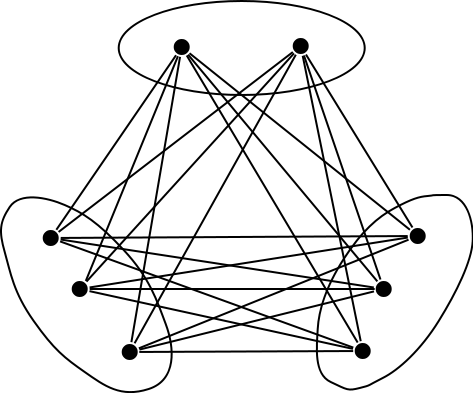
\includegraphics[width=5cm, height=5cm]{Turan.png}
\caption{Graf Tur\'ana $T(8,3)$}
    \label{Turan}
\end{figure}
\end{przy}

\begin{tw}[\textbf{Tur\'an, 1941}]
 Dla każdego $n\geq l$, każdy graf oparty na $n$ wierzchołkach, niezawierający  kliki $K_l$ i mający maksymalną
liczbę krawędzi jest grafem Tur\`ana T(n,l).
\end{tw}
Szczególnym przypadkiem powyższego twierdzenia (gdy $l$=2) jest twierdzenie Mantela:
\begin{tw}[\textbf{Mantel, 1907}]
 Maksymalna liczba krawędzi w grafie bez trójkątów jest równa co najwyżej $\lfloor \frac{n^2}{4} \rfloor$.
\end{tw}

\newpage

%-------------------------------ROZDZIAŁ II-----------------------------------------------------------------

\chapter{Twierdzenie Tur\`{a}na dla hipergrafów}
W rozdziale tym podamy definicje niezbędne do zrozumienia uogólnionego twierdzenia Tur\'ana. Przedstawimy również jeden z
jego kilku dowodów -- dłuższy, ale nieskomplikowany. Bardzo złożone hipergrafy ciężko, lub wręcz niemożliwe,
jest przedstawić graficznie w sposób jasny i przejrzysty, dlatego tylko najprostsze zostały umieszczone na rysunkach. 
Mam nadzieję, że jednak nie zniechęci to do wgłębienia się w jedną z ciekawszych działów matematyki- ekstremalną 
teorię hipergrafów. 
\section{Wprowadzenie do rozdziału}

Jeśli $V$ jest dowolnym zbiorem, to przez $|V|$ oznaczać będziemy liczność $V$, czyli liczbę elementów w $|V|$,
a przez $\mathcal{P}(V)$ zbiór wszystkich jego podzbiorów.\\
\begin{defi}
 \textbf{Hipergraf} jest uogólnieniem pojęcia grafu. To uporządkowana para \\
$H:=(V,E)$, gdzie:
\begin{itemize}
\item $V$ jest niepustym zbiorem, którego elementy nazywamy \textbf{wierzchołkami};
\item $E \subseteq \mathcal{P}(V)$. Elementy z $E$ nazywamy \textbf{hiperkrawędziami}, ale  dla ułatwienia nazywać je będziemy
po prostu krawędziami.
\end{itemize}
\end{defi}
Pojęcie hipergrafu utożsamiać będziemy ze zbiorem jego krawędzi. Mając na myśli zbiór wierzchołków hipergrafu, wyraźnie
to zaznaczymy. \\
\begin{defi}
 Dwa hipergrafy $H=(V,E)$ oraz $H'=(V',E')$ nazywamy \textbf{izomorficznymi}, jeśli istnieje bijekcja $f:V\rightarrow V'$
taka, że:\\
 $\{x_1,x_2,\dots,x_n\} \in E \Longleftrightarrow \{f(x_1),f(x_2),\dots,f(x_n)\} \in E'$
\end{defi}

\begin{defi}
 Hipergraf nazywamy \textbf{r-jednolitym}, jeśli każda jego krawędź ma liczność r.\\
\end{defi}
Zauważmy, że hipergraf 2-jednolity to po prostu graf.
Dla uproszczenia r-jednolity hipergraf będziemy nazywać r-grafem.\\
\begin{defi}
 \textbf{Podhipergrafem }hipergrafu $G=(V,E)$ lub hipergrafem \textbf{indukowanym} przez zbiór wierzchołków $N$ nazywamy hipergraf $H=(N,E')$, gdzie
$N \subseteq V(H)$, $E'\subseteq E$ oraz w $E'$ znajdują się tylko takie krawędzie, które zawierają wyłącznie wierzchołki z $N$.\\
Dla ułatwnienia będziemy nazywać go po prostu podhipergrafem.\\
\end{defi}
\begin{defi}
 Niech $\mathcal{F}$ będzie dowolną rodziną $r$-grafów, a $G$ dowolnym $r$-grafem. Mówimy, że $G$ jest \textbf{{$\mathcal{F}$}-wolny},
jeśli nie zawiera żadnego elementu z $\mathcal{F}$ jako podhipergrafu.
\\
\end{defi}

Przez \textbf{$ex(n,\mathcal{F})$} oznaczać będziemy maksymalną liczbę krawędzi w $n$ wierzchołkowym $r$-grafie $\mathcal{F}$-wolnym.\\
\begin{defi}
 Niech $l$,$r$ $\geq$2. Przez $K_l^{(r)}$ oznaczać będziemy rodzinę $r$-grafów z co najwyżej $l \choose 2$ krawędziami,
która zawiera zbiór wierzchołków $S$, zwany \textbf{rdzeniem}, taki, że:
\begin{itemize}
 \item |$S$|=$l$
 \item każda para wierzchołków z $S$ jest zawarta w jakiejś krawędzi.
\end{itemize}
\end{defi}

Zauważmy, że gdy $r$=2 to nasza rodzina $K_l^{(r)}$ redukuje się do grafu pełnego $K_l$. Dla $r$>2 $K_l^{(r)}$ zawiera więcej niż jeden $r$-graf.
Dla ustalonego $r$ i $l$ rodzina $K_l^{(r)}$ jest skończona, bo każdy jej element ma co najwyżej $l \choose 2$ krawędzi.\\
\begin{przy}
Na rysunku (\ref{rdzen}) przedstawiono hipergraf z rodziny $K_4^{(4)}$. Jego zbiór:
\begin{itemize}
 \item wierzchołków to $V=\{1,2,\dots,11\}$,
 \item krawędzi to  $E=\{ \{ 1,3,4,11\}, \{1,2,5,6\},\{2,4,6,7\},\{7,8,9,10\},\{2,3,10,11\}\}$
\end{itemize}
 Krawędzi jest 5, co jest mniejsze od $ {{l} \choose {2}}={{4}\choose{2}}=6$, a każda z nich jest mocy 4. Zbiór $S=\{1,2,3,4\}$
jest rdzeniem, gdyż $\{1,2\} \subset \{1,2,5,6\}$; $\{1,3\},\{1,4\}, \{3,4\} \subset \{ 1,3,4,11\}$;\\
$\{2,3\}\subset \{2,3,10,11\}$; $\{2,4\} \subset \{2,4,6,7\}$.


\begin{figure}[h]
\centering
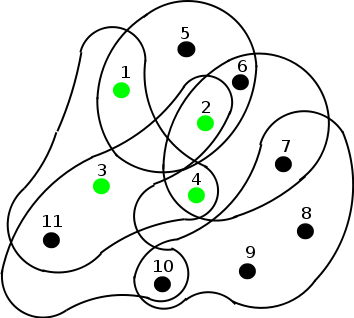
\includegraphics[width=5cm, height=5cm]{rdzen.png}
   \caption{Hipergraf z rodziny $K_4^{(4)}$ o rdzeniu $S=\{1,2,3,4\}$.}
    \label{rdzen}
\end{figure}
\end{przy}

\begin{defi}
  $r$-graf jest \textbf{$l$-dzielny}, jeśli zbiór jego wierzchołków można podzielić na $l$ podzbiorów (części) w taki sposób, aby
każda krawędź miała najwyżej jeden wierzchołek w każdym podzbiorze.
W szczególności, gdy $l$<$r$, to $r$-graf nie ma krawędzi.\\
$l$-dzielny $r$-graf nazywamy \textbf{pełnym}, gdy wszystkie dozwolone krawędzie są obecne.
\end{defi}
\begin{defi}
Niech $n$,$l$,$r$ $\geq 1$. Pełny $l$-dzielny $r$-graf oparty na $n$ wierzchołkach nazywamy \textbf{hipergrafem Tur\`{a}na},
jeśli liczność każdych dwóch części podziału różni się co najwyżej o 1. Taki hipergraf oznaczamy przez $T_r(n,l)$.
\end{defi}


Poszczególne części mają liczności:
\begin{center}
 $n_i=\lfloor \frac{n+i-1}{l}\rfloor$ dla $i \in [l]$
\end{center}
Liczba krawędzi w $T_r(n,l)$ to:
\begin{center}
 $t_r(n,l)=\sum \limits_{S \in {[l] \choose r}} \prod \limits_{i \in S} n_i$
\end{center}
Spośród wszystkich $l$-dzielnych $r$-grafów opartych na $n$ wierzchołkach hipergraf Tur\`{a}na $T_r(n,l)$ ma najwięcej krawędzi. 
W celu wyjaśnienia tego przeprowadzimy proste rozumowanie. Wiemy, że taki hipergraf $H$ na pewno musi być pełny. Liczba jego krawędzi 
będzie wyrażać się takim samym wzorem jak w przypadku hipergrafu Tur\'ana, czyli 
\begin{equation}
 |E(H)|=\sum \limits_{S \in {[l] \choose r}} \prod \limits_{i \in S} n_i
\end{equation}
gdzie $n_i$ to liczba wierzchołków w części i-tej, czyli
$n=n_1+n_2+\dots +n_l$.
Będzie to więc suma iloczynów liczności odpowiednich części. Nasze rozumowanie przeprowadzimy na
części $i$-tej i $j$ -tej ($i$,$j$ $\in [l]$) z podziału rozważanego hipergrafu, które mają liczności odpowiednio $n_i$ i $n_j$. Niech
części te różnią się o więcej niż jeden wierzchołek, więc bez straty ogólności załóżmy, że $n_i>n_j+1$. Zobaczmy, co się stanie
z iloczynem liczności części $i$-tej i $j$-tej,
jeśli wierzchołek z liczniejszej, $i$-tej części przerzucimy do $j$-tej. Liczba wierzchołków będzie dalej równa $n$, ponieważ
\begin{equation}
 n_1+n_2+\dots+(n_i-1)+\dots +(n_j+1)+\dots +n_l=n_1+n_2+\dots n_i+\dots +n_j+\dots +n_j=n
\end{equation}
Iloczyn ``nowej`` liczności części $i$-tej i $j$-tej w porównaniu do ''starej`` przedstawia się następująco:
\begin{equation}
(n_i-1)(n_j+1)=n_i \cdot n_j+n_i-n_j-1>n_i \cdot n_j+n_j+1-n_j-1=n_i \cdot n_j
\end{equation}
Oznacza to, że przerzucając wierzchołek z liczniejszej części podziału do mniej licznej, iloczyn się zwiększył, a tym samym 
wzrosła liczba krawędzi. Możemy więc wnioskować, że liczba krawędzi w takim hipergrafie będzie największa, jeśli wierzchołki
będą równomiernie rozłożone na $l$ części, czyli każde dwie części podziału mogą różnić się co najwyżej o 1, a to właśnie oznacza,
że jest to hipergraf Tur\'ana $T_r(n,l)$.

\begin{przy}
Na rysunku (\ref{hTuran}) przedstawiono hipergraf Tur\'ana $T_4(5,3)$. Jego zbiór pięciu wierzchołków został podzielony na 
3 części $n_i$ ($i=1,2,3$) zaznaczone symbolicznie niebieskimi elipsami: w dwóch częściach $n_1$,$n_2$ znajdują się po 2 wierzchołki, 
a w ostatniej, trzeciej $n_3$ tylko jeden. Wierzchołki znajdujące się w jednej części, zgodnie z definicją grafu Tur\'ana, 
nie mogą być połączone jakąkolwiek krawędzią.
\begin{figure}[h]
\centering
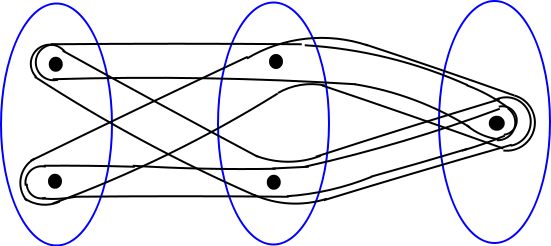
\includegraphics[width=10cm, height=4cm]{hTuran.png}
   \caption{Hipergraf Tur\'ana $T_4(5,3)$.}
    \label{hTuran}
\end{figure}
\end{przy}
\begin{defi}
 Niech $G$ będzie dowolnym $r$-grafem, a $x,y\in V(G)$, $x \not =y$. Wtedy:\\
\begin{itemize}
 \item$L_G(x)=\{S-\{x\} : x \in S\in G\}$ nazywamy \textbf{połączeniem} wierzchołka $x$;\\
 \item$deg_G(x)=|L_G(x)|$ nazywamy \textbf{stopniem} wierzchołka x;\\
 \item$codeg_G(x,y)$ nazywamy \textbf{stopniem pary} x,y i jest to liczba krawędzi w $G$, które zawierają jednocześnie $x$ i $y$;\\
 \item$N_G(x)=\{z:codeg_G(x,z)>0\}$ nazywamy \textbf{sąsiedztwem} lub \textbf{zbiorem sąsiadów} wierzchołka $x$ w $G$.
\end{itemize}
\end{defi}
Jeśli wiemy którego hipergrafu dotyczą powyższe określenia, wtedy dla przejrzystości zapisu indeks $G$ można pominąć.

\section{Twierdzenie Tur\'ana}
Twierdzenie, które jest tematem niniejszej pracy, nazywane jest rozszerzeniem twierdzeniem Tur\'ana, ponieważ jest sformułowane
dla hipergrafów, które, jak wcześniej zostało wspomniane, są uogólnieniami grafów. Twierdzenie podane w 1941 roku przez
P\'ala Tur\'ana jest więc szczególnym przypadkiem tego, które przedstawimy. Odpowiada ono na pytanie jaką maksymalną
liczbę krawędzi może posiadać $K_l^{(r)}$-wolny $r$-graf oparty na $n$ wierzchołkach. Znanych jest kilka dowodów tego twierdzenia,
jednak przedstawiony zostanie tylko jeden, oparty na dowodzie Erd\"osa z 1970 roku, ponieważ jest jasny, przejrzysty
i nie wymaga znajomości innych działów matematyki. Nim jednak do niego przejdziemy, przedstawimy lemat, z którego skorzystamy
w dowodzie twierdzenia Tur\'ana. 
\begin{lem} \label{lemat}
 Niech $n$ $\in \mathbb{N}$. Wtedy dla każdego $k \in [n]$ zachodzi:
\begin{equation}
t_r(n-k,l-1)+k \cdot t_{r-1}(n-k,l-1)\leq t_r(n,l) \label{nierownosc}
\end{equation}
Jeśli powyżej zachodzi równość, wtedy $k=\lfloor \frac{n}{l} \rfloor$ lub $k=\lceil \frac{n}{l} \rceil$.
\end{lem}
\begin{proof}
Niech $n$ $\in \mathbb{N}$. Dla każdego $k \in [n]$ lewą stronę nierówności można interpretować jako liczbę krawędzi w
następujacym hipergrafie: $T_r(n-k,l-1)$, do którego dokładamy $k$ wierzchołków, których połączenie jest hipergrafem
$T_{r-1}(n-k,l-1)$. Hipergrafy\\$T_r(n-k,l-1)$ i $T_{r-1}(n-k,l-1)$ oparte są na n-k wierzchołkach, podzielonych 
na $l-1$ części takich, że liczność każdych dwóch różni się co najwyżej o 1. To wszystko oznacza, że  podział ich wierzchołków jest
taki sam. Dzięki temu na lewą stronę nierówności można patrzeć jak na liczbę krawędzi w pełnym $l$-dzielnym $r$-grafie, 
którego każde dwie części spośród $l-1$ różnią się licznością o co najwyżej 1, a ostatnia, $l$-ta część, ma liczność $k$.
Jak już wcześniej zostało wspomniane, $T_r(n,l)$ maksymalizuje rodzinę pełnych $l$-dzielnych $r$-grafów, więc lewa strona
nierówności jest mniejsza od liczby krawędzi takiego hipergrafu oznaczanej przez $t_r(n,l)$. Jeśli w (\ref{nierownosc}) będzie zachodzić
równość, będzie to oznaczało, że $n$ wierzchołków zostało podzielonych na $l$ możliwie równych części, więc każde dwie części
będą się różniły o co najwyżej jeden wierzchołek, a to oznacza, że ostatnia ($l$-ta) część musi mieć liczność 
$\lfloor \frac{n}{l} \rfloor$ lub $\lceil \frac{n}{l} \rceil$.
\end{proof}
Warto zastanowić się, jak będzie wyglądał powyższy lemat gdy $l=r$. Ponieważ r>l-1, więc hipergraf $T_r(n-k,l-1)$ nie
będzie posiadał żadnej krawędzi, dlatego naszą nierówność można zredukować do:
\begin{equation}
k \cdot t_{r-1}(n-k,l-1)\leq t_r(n,l)
\end{equation}
Jeżeli powyżej będzie zachodzić równość, wtedy podobnie jak w dowodzie lematu, ostatnia $l$-ta część podziału zbioru wierzchołków
musi mieć liczność $\lfloor \frac{n}{l} \rfloor$ lub $\lceil \frac{n}{l} \rceil$.


\begin{tw}[\textbf{Tur\'ana}]\label{Turan}
Niech $n$,$l$,$r$ $\geq$ 2. Wtedy:
\begin{center}
$ex(n,K_{l+1}^{(r)}$)=$t_r(n,l)$\\
\end{center}
oraz jedynym $r$-grafem opartym na $n$ wierzchołkach, nie zawierającym elementu z $K_{l+1}^{(r)}$ jako podhipergrafu,
dla którego zachodzi powyższa równość to $T_r(n,l)$.\\
\end{tw}
\begin{proof}
 Przeprowadzimy dowód indukcyjny ze względu na $l$-liczbę części, na które został podzielony zbiór $n$ wierzchołków. Na początek
rozważymy najprostsze przypadki:
\begin{itemize}
 \item gdy $l<r$, wtedy $r$-graf nie ma żadnej krawędzi, więc na pewno jest $K_{l+1}^{(r)}$-wolny;
 \item gdy $r$=2, wtedy otrzymujemy twierdzenie Tur\'ana dla grafów;\\
Załóżmy więc, że $l\geq r>2$ i przez $G$ oznaczmy  $n$-wierzchołkowy $K_{l+1}^{(r)}$-wolny $r$-graf.
 \item gdy $n \leq l$, wtedy mamy kolejne 2 podprzypadki: $1^{\circ}$ $n<r$, wtedy hipergraf nie ma żadnej krawędzi, a tym
samym jest $K_{l+1}^{(r)}$-wolny; $2^{\circ}$ $n \geq r$, wtedy każdy spośród $n$ wierzchołków będzie znajdował się w innej
części podziału, ponieważ w ten sposób otrzymamy naj-\\ większą liczbę krawędzi, gdyż wierzchołki znajdujące się w tej samej części nie mogą
znaleźć się w jednej krawędzi. Maksymalną liczbę krawędzi jaką możę mieć ten $r$-graf to $n \choose r$, czyli $t_r(n,l)$. 
Jest on na pewno $K_{l+1}^{(r)}$-wolny, gdyż element z rodziny $K_{l+1}^{(r)}$ ma rdzeń rzędu $l+1$, a rozważany 
$r$-graf jest rzędu co najwyżej $l$.
\end{itemize}
Pomijając rozważone wyżej przypadki załóżmy, że $n\geq l+1\geq r+1>3$.\\
Niech $x \in V(G)$ będzie wierzchołkiem o maksymalnym stopniu $\Delta$, a przez $N=N(x)$ oznaczmy zbiór wszystkich sąsiadów 
wierzchołka $x$. Rozważmy $G[N]$, czyli $r$-graf indukowany przez zbiór wierzchołków $N$. Będziemy chcieli udowodnić, że
jest on $K_l^{(r)}$-wolny. W tym celu przeprowadzimy dowód niewprost. Załóżmy, że $G[N]$ zawiera jako podhipergraf element
z rodziny $K_l^{(r)}$, który oznaczymy przez $H$. Niech $S\subset V(H)$ będzie rdzeniem $H$, więc $|S|=l$. Tworzymy hipergraf $H'$ w
następujący sposób: do $H$ dodajemy wierzchołek $x$ oraz takie krawędzie, aby każda para wierzchołków $x$, $v$, gdzie $v\in S$
była zawarta w jakiejś z tych krawędzi. Jest to możliwe, ponieważ tak zdefiniowaliśmy zbiór $N$. Dodaliśmy więc co najwyżej $l$
krawędzi (bo taki rząd ma $S$), zbiór $S\cup \{x\}$ ma liczność $l+1$ i każda para z tego zbioru jest zawarta w jakiejś krawędzi, 
co oznacza, że jest to rdzeń. Hipergraf $|H'|$ ma co najwyżej ${{l+1} \choose 2}$ krawędzi, ponieważ:
\begin{equation}
 |H'| \leq |H|+l \leq {l \choose 2} + l={l \choose 2}+{l \choose 1}={{l+1} \choose 2}
\end{equation}
$H'$ jest więc elementem z rodziny $K_{l+1}^{(r)}$, co oznacza sprzeczność, ponieważ założyliśmy, że $G$ jest $K_{l+1}^{(r)}$-wolny,
a $H'$ jako jego podhipergraf również musi być $K_{l+1}^{(r)}$-wolny. $G[N]$ jest więc $K_l^{(r)}$-wolny.\\
Skupmy się teraz na $L(x)$, czyli połączeniu wierzchołka $x$. Będziemy chcieli udowodnić, że ten $(r-1)$-graf jest $K_l^{(r-1)}$-
wolny. Podobnie jak powyżej posłużymy się rozumowaniem niewprost. Załóżmy więc, że $L(x)$ zawiera jako podhipegraf element
z rodziny $K_l^{(r-1)}$, który oznaczmy przez $H$. Niech $S\subset V(H)$ będzie rdzeniem $H$, więc $|S|=l$. Tworzymy hipergraf
$H'$ poprzez dodanie do każdej krawędzi z $H$ wierzchołka $x$. Zbiór $S\cup \{x\}$ jest więc rdzeniem, $|H'|$ jest $r$-grafem,
który ma co najwyżej ${{l+1} \choose 2}$ krawędzi, ponieważ:
\begin{equation}
 |H'|=|H|\leq {l \choose 2} < {{l+1}\choose 2}
\end{equation}
$|H'|$ jest więc elementem rodziny $K_l^{(r-1)}$, co jest sprzeczne z naszym założeniem, że $G[N]$ jest $K_{l+1}^{(r)}$-wolny,
a $H'$ jako jego podhipergraf również musi być $K_{l+1}^{(r)}$-wolny. Oznacza to, że $L(x)$ jest $K_l^{(r-1)}$-wolny.\\
Ustalmy $k=n-|N|$. Z założenia indukcyjnego mamy:
\begin{itemize}
 \item $|G[N]|\leq t_r(n-k,l-1)$
 \item $\Delta = |L(x)|\leq t_{r-1}(n-k,l-1)$
\end{itemize}
Maksymalnym stopniem w $G$ jest $\Delta$, więc każdy wierzchołek w $V(G)-N$ ma stopień co najwyżej $\Delta$. Opierając się
na tym fakcie możemy wnioskować:
\begin{equation}
 |G|\leq|G[N]|+k\cdot \Delta\stackrel{zał.ind.}{\leq} t_r(n-k,l-1)+k\cdot t_{r-1}(n-k,l-1)
\stackrel{(\ref{nierownosc})}{\leq} t_r(n,l) \label{zaleznosc}
\end{equation}
Jeśli w powyższej zależności mamy
\begin{equation}
 t_r(n-k,l-1)+k\cdot t_{r-1}(n-k,l-1)= t_r(n,l)
\end{equation}
wtedy żadna krawędź w hipergrafie $G$ nie może zawierać dwóch wierzchołków ze zbioru $V(G)-N$, gdyż powodowałoby to
wielokrotne zliczanie krawędzi w pierwszej nierówności z  (\ref{zaleznosc}). Opierając się na lemacie (\ref{lemat}) 
wnioskujemy, że $k$ jest równe $\lfloor \frac{n}{l} \rfloor$ lub $\lceil \frac{n}{l} \rceil$.\\
Na podstawie indukcji wiemy, że $G[N]$ jest kopią hipergrafu $T_r(n-k,l-1)$, a połączenie każdego wierzchołka z $V(G)-N$
jest kopią $T_{r-1}(n-k,l-1)$. Rozważmy więc dwa przypadki:\\
$1^{\circ}$ $l>r$\\
Weźmy dowolne $z\notin N$. Połączenie $L(z)$ jest izomorficzne z hipergrafem Tur\'ana\\ $T_{r-1}(n-k,l-1)$. Jak wcześniej
ustaliliśmy żadna krawędź z $G$ nie ma dwóch wierzchołków w $V(G)-N$, więc elementami $L(z)$ są wyłączenie podzbiory $N$.
Pojawia się tutaj problem: czy podziały wierzchołków z $G[N]$ i $L(z)$ na l-1 części są takie same? 
Dowiedziemy, że tak własnie jest, stosując rozumowanie niewprost. W tym celu załóżmy, że $L(z)$ i $G[N]$ mają różne
podziały, które oznaczymy odpowiednio przez $V_1\cup V_2\cup \dots V_{l-1}$ oraz $W_1\cup W_2\cup \dots W_{l-1}$. 
Aby podziały te istotnie były różne, przyjmijmy, że $v_i \in V_i$, gdzie $i=1,2,\dots,l-1$ i jednocześnie 
$\{v_1,v_2\}\in W_1$. Na rysunku (\ref{d1}) schematycznie przedstawiono sytuację, ale aby nie zaciemniać  rysunku krawędzie
zostały pominięte.\\
Ponieważ wierzchołki $v_1$ i $v_2$ znajdują się w różnych częściach podziału w $L(z)$, to są połączone
krawędzią w $L(z)$, a więc również i w $G$ (krawędź w $L(z)$ wraz z wierzchołkiem $z$), czyli $codeg_G(v_1,v_2)>0$. 
Chwilowo skupimy się teraz na hipergrafie $G[N]$.\\
\begin{figure}[h]
\centering
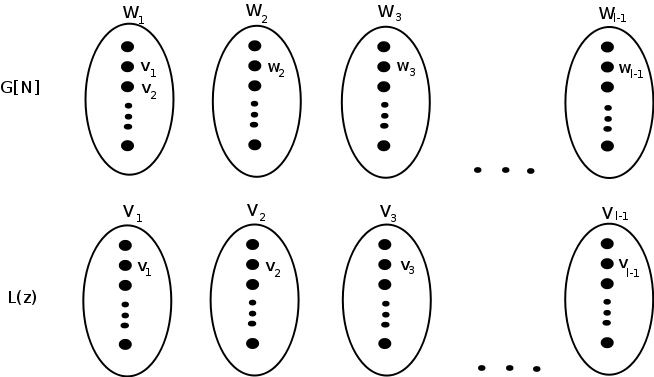
\includegraphics[width=12cm, height=6cm]{d1.png}
   \caption{Hipergrafy $G[N]$ i $L(z)$.}
    \label{d1}
\end{figure}
Załóżmy, że $w_j\in W_j$, gdzie $j\in \{2,3,\dots,l-1\}$ i 
oznaczmy $S=\{w_2,w_3,\dots,w_{l-1},v_1,v_2\}$.\\
Korzystając z wniosku, że $k=\lfloor \frac{n}{l} \rfloor$ lub $k=\lceil \frac{n}{l} \rceil$ oraz przyjętych założeń,
że $n \geq l+1$ i $l>r$ otrzymujemy następujące nierówności:
\begin{equation}
 n-k\geq n-\lceil \frac{n}{l} \rceil \geq (l+1)-2=l-1 \geq r
\end{equation}
Powyższe zależności gwarantują nam to, że $G[N]$ nie jest pusty, tzn. posiada co najmniej jedną krawędź, więc każde dwa
wierzchołki znajdujące się w różnych częściach podziału w $G[N]$ są połączone krawędzią w $G[N]$ (a więc i w $G$),
 co zapisujemy symbolicznie:dla $j \not =j'$ $codeg_{G[N]}(w_j,w_{j'})>0$ oraz dla $i=1,2$ $codeg_{G[N]}(w_j,v_i)>0$.
 Z wcześniejszego
wywodu wiemy,że $codeg_G(v_1,v_2)>0$. Oznacza to, że otrzymaliśmy element z rodziny $K_l^{(r)}$ o rdzeniu $S$. Dodając
wierzchołek $z$ otrzymamy hipergraf z rodziny $K_{l+1}^{(r)}$ o rdzeniu $S\cup \{z\}$, a to jest sprzeczne z założeniem, że
$G$ nie ma podhipergrafu z tej rodziny. $L(z)$ ma więc taki sam podział jak $G[N]$, a rozważany  $G$ jest hipergrafem
Tur\'ana $T_r(n,l)$.\\
$2^{\circ}$ $l=r$\\
W tym przypadku $G[N]$ nie ma żadnej krawędzi, więc nie można przeprowadzić takiego rozumowania jak w $1^{\circ}$. W tym
przypadku będziemy chcieli udowodnić, że dla dowolnych dwóch wierzchołków $z, z'$ ze zbioru $V(G)-N$, połączenia
$L(z)$ oraz $L(z')$ mają takie same $(l-1)$-podziały. Podobnie jak w $1^{\circ}$ przeprowadzimy rozumowanie niewprost. 
W tym celu załóżmy, że podziały te są różne i oznaczmy je odpowiednio przez $V_1\cup V_2\cup \dots V_{l-1}$ oraz $W_1\cup 
W_2\cup \dots W_{l-1}$. Załóżmy, że $v_i \in V_i$, gdzie $i=1,2,\dots,l-1$ i jednocześnie 
$\{v_1,v_2\}\in W_1$. $v_1$ i $v_2$ znajdują się w różnych częściach podziału w $L(z')$, więc istnieje w $L(z')$, a tym 
samym w $G$, krawędź która je zawiera. Dodając do tego fakt, że \\
$j \not =j'$ $codeg_{G[N]}(w_j,w_{j'})>0$ oraz dla
 $i=1,2$ $codeg_{G[N]}(w_j,v_i)>0$ otrzymujemy element z rodziny $K_l^{(r)}$ o rdzeniu $S=\{w_2,w_3,\dots,w_{l-1},v_1,v_2\}$.
Dokładając wierzchołek $z$ mamy kopię hipergrafu z $K_{l+1}^{(r)}$ o rdzeniu $S\cup \{z\}$, co jest sprzeczne z przyjętym
założeniem, że $G$ takiej nie posiada, dlatego $L(z)$ musi mieć taki podział jak $L(z')$, a $G$ jest hipergrafem
Tur\'ana $T_r(n,l)$.
\end{proof}
\chapter{Problem Tur\'ana}
Przedstawione w poprzednim rozdziale twierdzenie Tur\'ana odpowiada na jedno z wielu pytań, którymi zajmuje się ekstremalna
teoria hipergrafów. Zagadnienia, które zostaną poruszone w tym rozdziale związane są z gęstością Tur\'ana. Nim jednak do nich
przejdziemy, niezbędne jest wprowadzenie kilku definicji i oznaczeń.\\
Przez $K_k(l)$ oznaczać będziemy $k$-jednolity hipergraf oparty na $l$ wierzchołkach, który posiada wszystkie możliwe krawędzie.
Zauważmy, że gdy $k=2$, $K_k(l)$ redukuje się do grafu pełnego o $l$ wierzchołkach.
\begin{defi}
 \textbf{Gęstością Tur\'ana} $\pi (H)$ dla $k$-jednolitego hipergrafu $H$ nazywamy wyrażenie:
\begin{equation}
 \pi(H)=\lim_{n \to \infty} \frac{ex(n,H)}{{n \choose k}}
\end{equation}

gdzie $ex(n,H)$ jest maksymalną liczbą krawędzi w $n$ wierzchołkowym $H$-wolnym $k$-grafie.
\end{defi}
Jest to więc stosunek maksymalnej ilości krawędzi w $n$ wierzchołkowym $H$-wolnym $k$-grafie do maksymalnej liczby krawędzi
jaką może posiadać $k$-graf. Wiadomo, że gęstość nie wzrasta ze wzrotem $n$, a dla każdego $k$ i $l$ $ \pi(K_k(l))$ istnieje,
 jednak nie wiadomo ile ona wynosi dla $l>k\geq 3$. Wielu matematyków
podjęło, z różnymi skutkami, wyzwanie wyznaczenia wartości $\pi$ dla poszczególnych rodzin hipergrafów. P\'al Tur\'an pracował
m.in. nad odpowiedzią na pytanie jaki maksymalny rozmiar może mieć 3-jednolity hipergraf, aby nie zawierał $K_3(4)$ jako
podhipergrafu. Podał on dowód-konstrukcję, która świadczyła o tym, że $\pi(K_3(4))\geq \frac{5}{9}$. Przypuszczał on także, 
że jest najlepsze ograniczenie, jednak nikt tego przypuszczenia ani nie obalił ani nie potwierdził, więc problem
pozostał wciąż otwarty. Przypadkiem tym zajęło się wielu matematyków i owszem, znaleźli inne nieizomorficzne hipergrafy, jednak
wszystkie miały dokładnie ten sam rozmiar, co skonstruowane przez Tur\'ana. Dopiero Chung i Lu znaleźli lepsze ograniczenie 
na $\pi(K_3(4))$ i udowodnili, że wartość ta jest większa od $\frac{\sqrt{21}-1}{6}$.\\
W miarę rozwoju ekstremalnej teorii hipergrafów pojawiały się coraz nowsze problemy do rozwiązania. Jednym z nich było 
pytanie jaka jest maksymalna liczba krawędzi w $k$-grafie opartym na $n$ wierzchołkach takim, że różnica symetryczna
każdych dwóch różnych krawędzi nie zawiera się w żadnej innej krawędzi? Zapiszmy to formalnie. 
\begin{defi}
 \textbf{Różnicą symetryczną} dwóch zbiorów $A$ i $B$ nazywamy operację:
\begin{equation}
 A\triangle B=(A\setminus B)\cup (B\setminus A)
\end{equation}
\end{defi}
Przez $\mathcal{D}_k$ oznaczmy rodzinę $k$-jednolitych hipergrafów, której dowolny zbiór trzech różnych krawędzi $\{A,B,C\}$
spełnia zależność: $A\triangle B\subseteq C$, czyli różnica symetryczna każdych dwóch różnych krawędzi jest zawarta
w co najmniej jednej, innej krawędzi.
B\'ela Ballob\'as, węgierski matematyk postawił następującą hipotezę:
\begin{hip}\label{hipoteza}
$ex(n,\mathcal{D}_k)=\lfloor \frac{n}{k} \rfloor \cdot \lfloor \frac{n+1}{k} \rfloor \cdot$ $\dots$ $\cdot \lfloor \frac{n+k-1}{k} \rfloor$
\end{hip}
Próbę udowodnienia bądź obalenia powyższej hipotezy podjęło wielu matematyków. Frankl i F\"{u}redi udowodnili ja dla $n\geq 2k$,
Ballob\'as dla $k=3$, a Sidorenko dla $k=4$. Poniżej znajduje się przykład dla $k=3$ i $n=5$.
\begin{przy}
Niech $k=3$, $n=5$, więc $5\geq 2\cdot 3 =6$, wtedy $ex(5,\mathcal{D}_3)=\lfloor \frac{5}{3} \rfloor \cdot \lfloor \frac{6}{3} \rfloor \cdot
 \lfloor \frac{7}{3} \rfloor=1\cdot 2\cdot 2 =4$, czyli rozważany 3-graf, według Frankla i F\"{u}redi'ego, może mieć maksymalnie
4 krawędzie, aby nie zawierał $\mathcal{D}_3$ jako podhipergrafu.\\
Określmy hipergraf następująco: $H=\{\underbrace{\{1,3,5\}}_{A},\underbrace{\{1,4,5\}}_{B},\underbrace{\{2,3,5\}}_{C}, 
\underbrace{\{2,4,5\}}_{D}\}$. Dla ułatwienia krawędzie oznaczono literami A,B,C,D. $H$ nie zawiera $\mathcal{D}_3$, ponieważ:\\ 


\begin{tabular}{l l}
$ A \triangle B=\{3,4\}\not \subseteq C,D$,& $ A \triangle C=\{1,2\}\not \subseteq B,D$,\\
$ A \triangle D=\{1,2,3,4\}\not\subseteq B,C$, & $ B \triangle C=\{1,2,3,4\}\not \subseteq A,D$,\\
$ B \triangle D=\{1,2\}\not \subseteq A,C$, & $ C \triangle D=\{3,4\}\not \subseteq A,B$.
\end{tabular}\\
Zauważmy, że dodanie jakiejkolwiek krawędzi o liczności 3 spowoduje pojawienie się $\mathcal{D}_3$.
\end{przy}

Dominique de Caen postawił kolejne pytanie związane w ekstremalną teorią hipergrafów:jaka jest maksymalna liczba krawędzi w
$k$-grafie, który nie zawiera żadnej trójki krawędzi $\{A,B,C\}$ takiej, że $|A \cap B|=k-1$ oraz $A \triangle B \subseteq C$. 
Zapiszmy ten problem formalnie. Niech $\mathcal{A}_i=\{\{1,2,\dots,k\},\{1,2,\dots,k-1,k+1\},\{i,i+1,\dots,i+k-1\}\}$
oraz\\
$\mathcal{S}_k=\{\mathcal{A}_2,\mathcal{A}_3,\dots,\mathcal{A}_k\}$. Szukamy więc $ex(n,\mathcal{S}_k)$. Wspomniany wyżej 
Sidorenko rozwiązał ten problem dla $k=3,4$:
\begin{tw}\label{Sidorenko}
 Dla $k=3$ i $k=4$, $ex(n,\mathcal{S}_k)=\lfloor \frac{n}{k} \rfloor \cdot \lfloor \frac{n+1}{k} \rfloor 
\cdot$ $\dots$ $\cdot \lfloor \frac{n+k-1}{k} \rfloor$.
\end{tw}
Rodzina $\mathcal{S}_k$ jest szczególnym przypadkiem $\mathcal{D}_k$, więc hipoteza (\ref{hipoteza}) dla $k=3,4$ wynika z
powyższe twierdzenia (\ref{hipoteza}):
\begin{equation}
 \lfloor \frac{n}{k} \rfloor \cdot \lfloor \frac{n+1}{k} \rfloor 
\cdot \dots \cdot \lfloor \frac{n+k-1}{k} \rfloor \leq ex(n, \mathcal{D}_k) \leq ex(n, \mathcal{S}_k)
\end{equation}



\end{document}
